\listfiles
\documentclass[a4paper, oneside]{report}

\usepackage[utf8]{inputenc}
\usepackage[francais]{babel}

\usepackage{amssymb}

\usepackage[pdftex]{graphicx}
\usepackage{graphics}

\usepackage[top=3cm, bottom=2cm, left=3cm, right=2cm]{geometry}

\usepackage{multirow}
\usepackage{tabularx}

\usepackage{listings} % a inclure pour la fonction listing
\usepackage{color} % on en a besoin pour utiliser les couleurs
\definecolor{grey}{rgb}{0.95,0.95,0.95} % on definit la couleur grise (c'est un gris tres clair)
		
\usepackage{float}

\renewcommand{\floatpagefraction}{.9} 
%utilisee avec la commande :
\renewcommand{\textfraction}{.1}
%permet de dire que le texte peut n'occuper que 10% d'une
%page, et donc que des flottants peuvent occuper les 90% restant.


%Il y a d'autres parametres interessants :
\setcounter{totalnumber}{4} 
\setcounter{secnumdepth}{3}
%qui determine le nombre de flottants autorises par page,
\renewcommand{\topfraction}{.8}
\renewcommand{\bottomfraction}{.8}

\lstset{numbers=left, tabsize=2, frame=single, breaklines=true, basicstyle=\ttfamily, numberstyle=\tiny\ttfamily, framexleftmargin=13mm, backgroundcolor=\color{grey}, xleftmargin=12mm}

% titre du document
\title{IN41 \\ TP2 :  Echantillonnage}
% auteur du document
\author{Ripard Maxime}

\begin{document}
  \maketitle
  \newpage{}
  \tableofcontents
  \newpage{}


  \chapter{Introduction}
    \section{Code}
    
  \begin{lstlisting}
lambda=1000; % Parametre (1000 ou 2000)
Fe=8000; % Freq. echantillonnage
F0=1000; % Freq. de depart
T=2; % Duree d'observation
it=(0:Fe*T-1)/Fe; % Vecteur temps
theta=2*pi*F0*it+pi*lambda*(it .^2);
x=cos(theta);
soundsc(x,Fe); % Ecoute
\end{lstlisting}
  
  \section{Interpr\'etation}
  
La fonction de $\lambda$ est une somme de sinuso\"ides contenant l'information du signal analogique d'origine.
Quand $\lambda=1000$, nous pouvons entendre une mont\'ee assez lin\'eaire vers les aigus et donc en fr\'equence. 
Lorsque $\lambda=2000$, nous entendons cette m\ˆeme mont\'ee vers les aigus, plus rapide toutefois, puis une descente vers les graves vers la fin.
\\
Si on utilise $\lambda=3000$, cela confirme ce que nous pensions avec $\lambda=2000$, nous avons une redescente franche vers les graves. On peut supposer que si on continue d'augmenter encore $\lambda$, on aura une remont\'ee vers les aigus, produisant ainsi une sinuso\¨ide.
\\
\\
Si nous prenions un vecteur temps plus long, nous aurions surement plusieurs répétitions de la sinuso\¨ide, le signal \'etant une somme de sinuso\¨ides.
\\
\\
Le principe que nous cherchons \`a mettre en avant est nettement visible pour $\lambda=3000$.\\
En effet, ce dernier nous permet d'introduire le th\'eor\`eme de Shannon :
\\
\\
Le th\'eor\`eme de Nyquist-Shannon dis qu'une fr\'equence d'\'echantillonnage d'un signal doit \ˆetre au moins \'egale au double de la fr\'equence de ce signal, afin de convertir ce signal d'une forme analogique \`a une forme num\'erique. Ce th\'eor\`eme est \`a la base de la conversion num\'erique des signaux et s'applique donc dans des domaines aussi vari\'es que l'audio, la t\'el\'ephonie, etc...

\newpage{}
\chapter{Th\`eme d'\'etude}
 \section{Repr\'esentation d'un signal r\'eel}
 	\subsection{Code}
	
  \begin{lstlisting}
f0 = 10;
t=[-2:0.001:2];
x = f0*sincard(pi*f0*t);
plot(t,x);
end
\end{lstlisting}  
  
 	\subsection{Repr\'esentation graphique}

\begin{figure}[h]
   \centering
    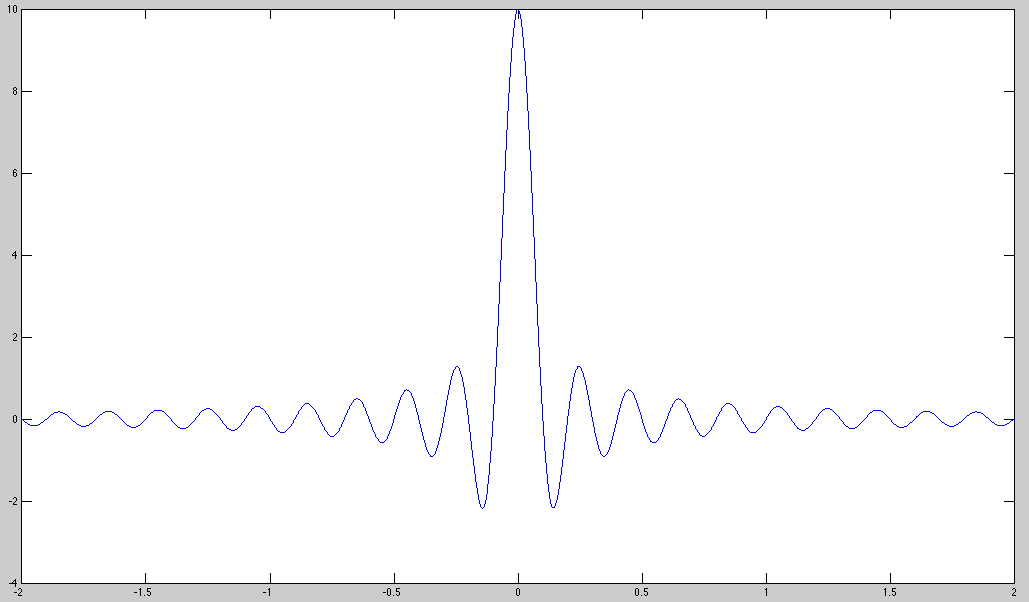
\includegraphics[scale=0.40]{images/exo1.png}
    \caption{Repr\'esentation d'un signal x(t)}
  \end{figure}
  
  \newpage{}
  \section{Echantillonnage}
  \subsection{Echantillonnage id\'eal}
    \subsubsection{Code}
	 \begin{lstlisting}

f = [ 5 10 30];
f0=10;
for i=1:3

    t=(min:1/f(i):max);

    x=f0*sincard(pi*f0*t);

    figure(2)
    subplot(3,1,i);
    plot(t,x)
    grid
    axis([-2 2 -2 10])
     switch i                                
        case 1, legend('5 Hz')       
        case 2, legend('10 Hz')    
        case 3, legend('30 Hz')
     end
end
end
\end{lstlisting}  
	
	\subsubsection{Repr\'esentation graphique}

\begin{figure}[h]
   \centering
    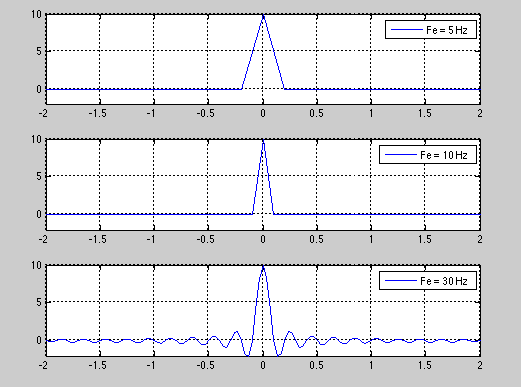
\includegraphics[scale=0.80]{images/Exo2.png}
    \caption{Repr\'esentation des signaux id\'eaux}
  \end{figure}
 	\newpage{} 
  	\subsubsection{Interpr\'etation}
	
	Comme nous l'avons vu pr\'ec\'edemment, pour qu'un signal ne soit pas affecté par un \'echantillonage, il faut que la fr\'equence d'\'echantillonage soit le double de la fr\'equence maximale du signal.\\
	\\
	Dans cet exercice, la fr\'equence maximale est $f0=10Hz$.\\
	Pour avoir un \'echantillonnage correct, il faut donc que notre fr\'equence d'\'echantillonnage soit au minimum au double de f0, soit 20Hz.\\
	Ceci est d'ailleurs justifi\'e par les courbes. La premi\`ere est pauvre en informations par rapport au signal d'origine, la deuxi\`eme \'egalement, cependant la troisi\`eme pr\'esente une belle sinuso\¨ide. La seule diff\'erence r\'eside dans le fait que la fr\'equence d'\'echantillonage respecte ou non le th\'eor\`eme de Shannon.\\
\\

  
  \newpage{}
 \subsection{Echantillonnage r\'eel}
 	\subsubsection{Code}
	
	 \begin{lstlisting}
%arguments
dt=1/120;
nbel=5;
max=-min=2;


fe = [5 10 30];
f0 = 10;

for i=1:3
    t=[min:1/fe(i):max]; % Construction des vecteurs en fonctions des arguments
    x = length((max-min)*fe(i));
    j=1;
    for l = t
        ts=[l:dt/nbel:l+dt];
        xs=f0*sincard(pi*f0*ts);
        x(j) = mean(xs); %Construction de x(t)
        j=j+1;
    end
    
    figure(3)
    subplot(3,1,i)
    plot(t,x)
    grid
    axis([-2 2 -2 10])
    switch i                                
        case 1, legend('Fe = 5 Hz')       
        case 2, legend('Fe = 10 Hz')    
        case 3, legend('Fe = 30 Hz')
    end
end
    \end{lstlisting}  
	
	\newpage{}
	\subsubsection{Repr\'esentation graphique}
	
	\begin{figure}[h]
   \centering
    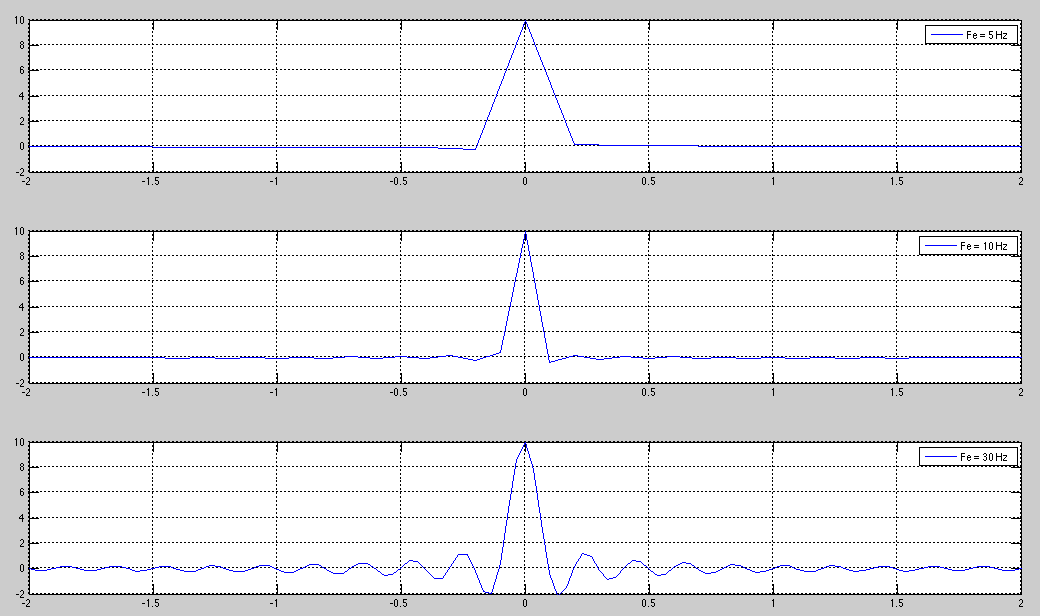
\includegraphics[scale=0.43]{images/Exo3.png}
    \caption{Repr\'esentation des signaux r\'eels}
  \end{figure}
  
	\subsubsection{Interpr\'etation}
	Pour obtenir un échantillonage des signaux r\'eels, on utilise ici une impulsion de largeur finie, en consid\'erant la valeur moyenne du signal pendant la durée de l'impulsion. Ceci est une vision contraire aux signaux id\'eaux, qui eux sont \'echantillonn\'es en tenant compte d'une impulsion infiniment courte d'un peigne de Dirac. Les signaux dans la r\'ealit\'e sont consid\'er\'es comme r\'eels, car l'\'echantillonnage ne peut \ˆetre consid\'er\'e comme \'etant instantan\'e.
	\\
	Cependant, a l'instar des signaux id\'eaux, le th\'ero\`eme de Shannon s'applique \`a l'\'echantillonnage. \\
	De plus, plus $\Delta t$ tend vers 0, plus notre signal r\'eel s'approche d'un signal id\'eal. On doit donc utiliser un $\Delta t$ le plus petit possible.
	\\
	\\
	Dans cet exemple, on choisit donc un $\Delta t = 1/120$, correspondant \`a un quart de la p\'eriode d'\'echantillonnage.
	
	\newpage{}
	\section{Reconstruction par extrapolation d'ordre 0}
 	\subsection{Code}
	
	 \begin{lstlisting}
Arguments :
fe = 10 Hz
dt = 1/120
nbel = 5
min =-2
max = 2
extrapaccuracy = 10

...
	 
ti = [min:1/fe:max]; %Cr\'eation des vecteurs n\'ecessaires
tr = ti;

tsi = [min:1/(extrapaccuracy*fe):max];
tsr = [min:1/(extrapaccuracy*fe):max];

xi = idealsampling(fe,min,max);
xr = realsampling(fe,dt,nbel,min,max);

xsi = length(tsr);
xsr = length(tsr);

k=1;
l=1;
for i = ti
    if (l ~= size(xi))
        for j = 0:(extrapaccuracy-1)
          xsi(j+k) = xi(l); %Comblage avec les valeurs constantes
          xsr(j+k) = xr(l);
        end
    else
        xsi(k) = xi(l);
        xsr(k) = xr(l);
    end
    k = k+extrapaccuracy;
    l = l+1;
end
figure(1);
subplot(2,1,1)
plot(tsr,xsr)
title('Echantillonage Reel')
grid
axis([min max -2 11]);
subplot(2,1,2)
plot(tsi,xsi)
title('Echantillonage ideal')
grid
axis([min max -2 11]);
end
    \end{lstlisting}  
	
	\newpage{}
	\subsection{Repr\'esentation graphique}
	
	\begin{figure}[h]
   \centering
    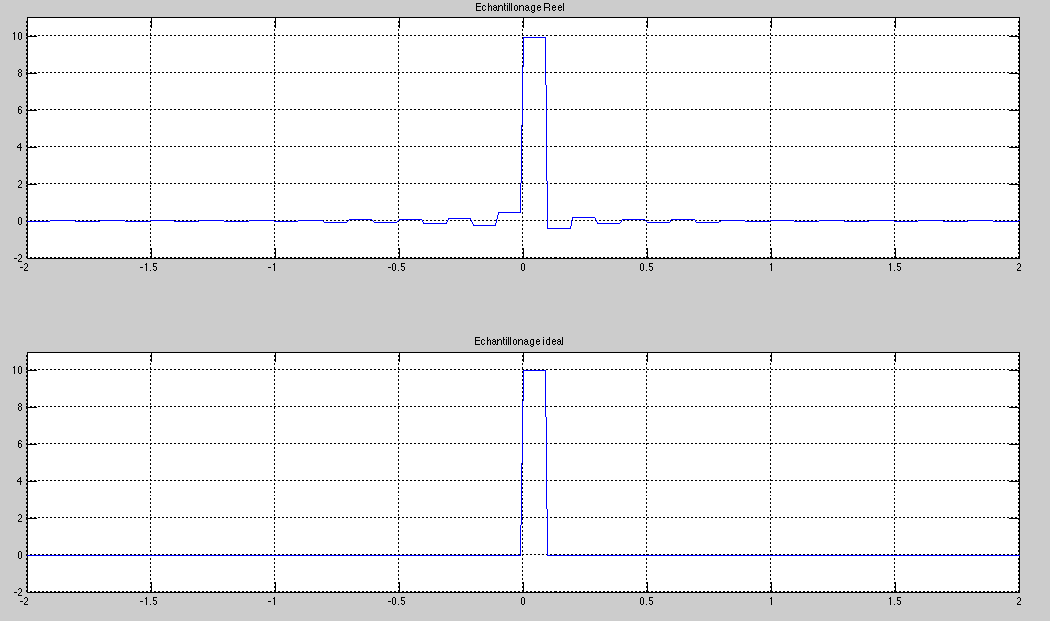
\includegraphics[scale=0.43]{images/Exo4_0.png}
    \caption{Representation des signaux id\'eaux et r\'eels reconstruits par extrapolation d'ordre 0}
  \end{figure}
  
	\subsection{Interpr\'etation}
	
Lorsqu'un signal \'echantillonn\'e subit une extrapolation d'ordre 0, on bloque le signal \`a sa valeur jusqu'\`a la r\'ecup\'eration de la valeur suivante. Ainsi, le signal reconstitu\'e pr\'esente un effet de scaling. Cependant, on peut essayer de limiter ce phénomène en augmentant la fréquence d'échantillonnage, ayant ainsi moins \`a "combler" le signal lors de son extrapolation.\\
Nous avons ici volontairement choisi une fr\'equence d'\'echantillonnage faible relativement \`a la fr\'equence du signal pour mettre en \'evidence les d\'efauts de l'\'echantillonnage.

\newpage{}
\section{Reconstruction par extrapolation d'ordre 1}
	\subsection{Code}
	 \begin{lstlisting}
Arguments :
fe = 10 Hz
dt = 1/120
nbel = 5
min =-2
max = 2
extrapaccuracy = 10

...
	 
ti = [min:1/fe:max]; %Cr\'eation des vecteurs
tr = ti;

tsi = [min:1/(extrapaccuracy*fe):max];
tsr = [min:1/(extrapaccuracy*fe):max];

xi = idealsampling(fe,min,max);
xr = realsampling(fe,dt,nbel,min,max);

xsi = length(tsr);
xsr = length(tsr);

k=1;
l=1;
for i = ti
    if (l ~= size(xi))
        tmpi = (xi(l+1)-xi(l))/extrapaccuracy; %Determination du pas d'incr\'ement
        tmpr = (xr(l+1)-xr(l))/extrapaccuracy;
        for j = 0:(extrapaccuracy-1)
          xsi(j+k) = xi(l)+tmpi*j; %Comblage avec les valeurs incr\'ement\'ees
          xsr(j+k) = xr(l)+tmpr*j;
        end
    else
        xsi(k) = xi(l);
        xsr(k) = xr(l);
    end
    k = k+extrapaccuracy;
    l = l+1;
end
figure(1);
subplot(2,1,1);
plot(tsr,xsr);
subplot(2,1,2);
plot(tsi,xsi);
end
\end{lstlisting} 

\newpage{}
\subsection{Repr\'esentation graphique}
	
	\begin{figure}[h]
   \centering
    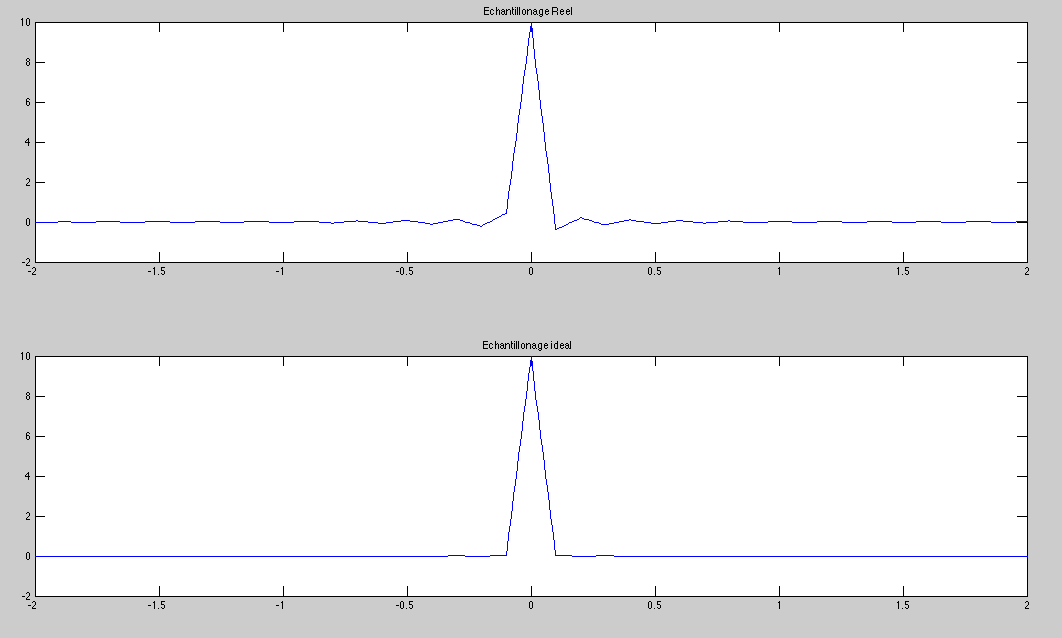
\includegraphics[scale=0.43]{images/Exo4_1.png}
    \caption{Representation des signaux r\'eels reconstruits par extrapolation d'ordre 1}
  \end{figure}

\subsection{Interpr\'etation}

L'extrapolation d'ordre 1 comble les valeurs manquantes par une droite l\`a o\`u l'extrapolation d'ordre 0 comblait par les m\ˆemes valeurs. Cette extrapolation permet donc de supprimer les effets de scaling pr\'esents dans l'\'echantillonage d'ordre 0.\\
Il est donc globalement plus précis.

\section{Conclusion}

Nous avons vu qu'un \'echantillonnage doit respecter le th\'eor\`eme de Shannon pour qu'il soit d'une qualit\'e acceptable.\\

De plus, on a remarqu\'e que la m\'ethode d'\'echantillonnage est aussi un crit\`ere de qualit\'e, en augmentant l'ordre de la m\'ethode, on augmente aussi l'efficacit\'e de la reconstruction.  
\end{document}